\documentclass[tikz,border=8pt]{standalone}
\usetikzlibrary{arrows.meta,positioning,fit}
\begin{document}
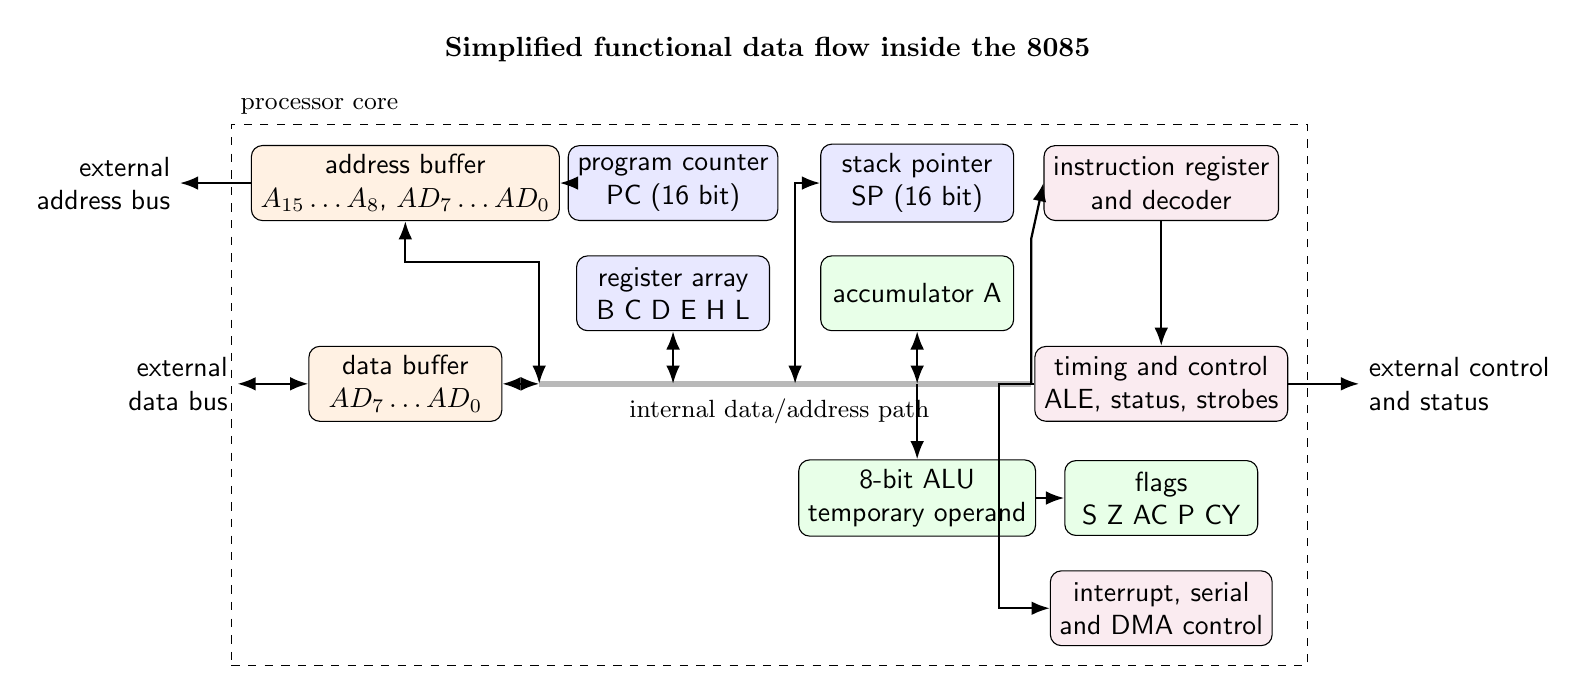
\begin{tikzpicture}[
  font=\sffamily,
  >=Latex,
  block/.style={draw,rounded corners,minimum width=2.45cm,minimum height=0.95cm,align=center},
  flow/.style={->,thick},
  biflow/.style={<->,thick}
]
\node[font=\bfseries] at (6.2,4.25) {Simplified functional data flow inside the 8085};

\node[block,fill=orange!11] (abuf) at (1.6,2.55) {address buffer\\$A_{15}\ldots A_8$, $AD_7\ldots AD_0$};
\node[block,fill=orange!11] (dbuf) at (1.6,0) {data buffer\\$AD_7\ldots AD_0$};
\node[left=9mm of abuf,align=right] (aext) {external\\address bus};
\node[left=9mm of dbuf,align=right] (dext) {external\\data bus};

\node[block,fill=blue!9] (pc) at (5.0,2.55) {program counter\\PC (16 bit)};
\node[block,fill=blue!9] (sp) at (8.1,2.55) {stack pointer\\SP (16 bit)};
\node[block,fill=blue!9] (regs) at (5.0,1.15) {register array\\B C D E H L};
\node[block,fill=green!9] (acc) at (8.1,1.15) {accumulator A};
\node[block,fill=green!9] (alu) at (8.1,-1.45) {8-bit ALU\\temporary operand};
\node[block,fill=green!9] (flags) at (11.2,-1.45) {flags\\S Z AC P CY};

\node[block,fill=purple!8] (ir) at (11.2,2.55) {instruction register\\and decoder};
\node[block,fill=purple!8] (tim) at (11.2,0) {timing and control\\ALE, status, strobes};
\node[block,fill=purple!8] (ints) at (11.2,-2.85) {interrupt, serial\\and DMA control};
\node[right=9mm of tim,align=left] (cext) {external control\\and status};

\draw[line width=2.1pt,gray!55] (3.3,0) -- (9.55,0);
\node[below=2pt,font=\small] at (6.35,0) {internal data/address path};

\draw[flow] (abuf) -- (aext);
\draw[flow] (pc.west) -- (abuf.east);
\draw[biflow] (dext) -- (dbuf);
\draw[biflow] (dbuf.east) -- (3.3,0);
\draw[biflow] (3.3,0) -- (3.3,1.55) -| (abuf.south);
\draw[biflow] (sp.west) -- (6.55,2.55) -- (6.55,0);
\draw[biflow] (regs.south) -- (5.0,0);
\draw[biflow] (acc.south) -- (8.1,0);
\draw[flow] (8.1,0) -- (alu.north);
\draw[flow] (alu) -- (flags);
\draw[flow] (9.55,0) -- (9.55,1.85) -- (ir.west);
\draw[flow] (ir) -- (tim);
\draw[flow] (tim) -- (cext);
\draw[flow] (tim.west) -- ++(-0.45,0) |- (ints.west);

\node[draw,dashed,fit=(abuf)(dbuf)(pc)(sp)(regs)(acc)(alu)(flags)(ir)(tim)(ints),inner sep=7pt] (chip) {};
\node[above right,font=\small] at (chip.north west) {processor core};
\end{tikzpicture}
\end{document}
